% !TeX encoding = UTF-8
% !TeX spellcheck = de_DE
\section{FPGAs und Hardwarebeschreibung}
\subsection{Aufbau und Struktur eines FPGAs}
Ein FPGA  (\textbf{F}ield \textbf{P}rogrammable \textbf{G}ate \textbf{A}rray) ist ein frei programmierbarer Logikschaltkreis, welcher aus einer Matrix-Struktur aus konfigurierbaren Logikblöcken besteht. Diese Logikblöcke werden auch als CLB (\textbf{C}onfigurable \textbf{L}ogic \textbf{B}locks) bezeichnet. Die CLBs wiederum bestehen unter anderem aus SRAM\footnote{\textbf{S}tatic \textbf{R}andom \textbf{A}ccess \textbf{M}emory, Statisches RAM}-Blöcken, welche die während des Hardwareentwurfs entwickelten Logikfunktionen umsetzen. Für die Kommunikation mit der Außenwelt dienen die am FPGA existierenden Ein- und Ausgabeblöcke (I/O-Blöcke).

\begin{figure}[H]
	\centering
	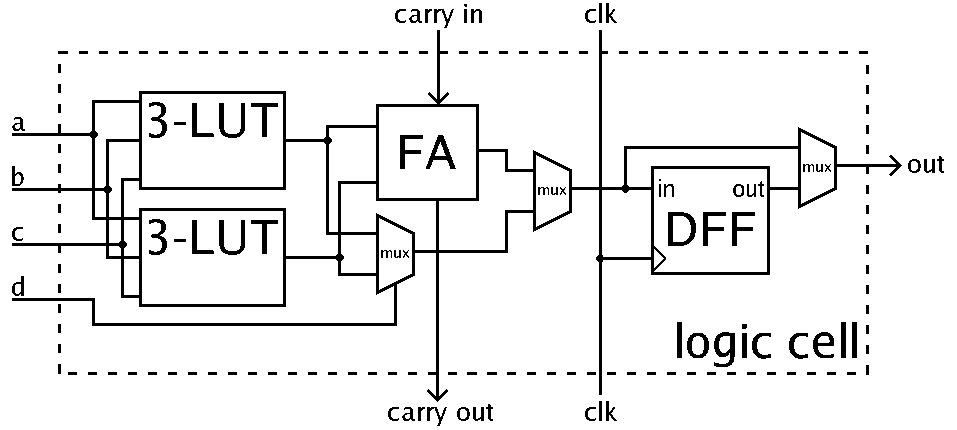
\includegraphics[width=0.75\linewidth]{img/verilog/clb.png}
	\caption{CLB \cite{clb_IMG}}
	\label{fig:clb}
\end{figure}

Jede CLB besitzt feste Bestandteile wie z.B. Lookup"=Tabellen (LUT) und Flipflops, auf welche der Hardwareentwurf abgebildet werden kann. Besonderheit der Lookup"=Tabellen ist, dass diese zur Realisierung von Logik-Operationen wie z.B. AND, OR, NOT oder XOR oder im Spezialfall als RAM (\textbf{R}andom \textbf{A}ccess \textbf{M}emory) genutzt weden können. Ein FPGA besteht aus einer großen Anzahl Logikzellen, deren Gesamtkapazität in der Größe "`Gatteräquivalente"' angegeben wird. \\
Beispielsweise hat das hier verwendete Spartan 3E FPGA zwei 4-bit-input LUTs und zwei Flip Flops. Ein Kintex 7 hingegen hat vier 6-bit-input LUTS und acht Flip Flops. Beide haben außerdem weitere carry und arithmetische Logik, sowie Multiplexer.


Für die Erstellung von Hardwareentwürfen für FPGAs werden Entwurfswerkzeuge benötigt. Die eigentliche Erstellung des Entwurfs erfolgt unter Verwendung von Hardwarebeschreibungssprachen wie die anschließend vorgestellte Verilog oder VHDL. Solche Hardwarebeschreibungssprachen arbeiten nicht mit einzelnen elektronischen Bauteilen, sondern beschreiben das gewünschte Verhalten einer Schaltung auf einem anderen Abstraktionsebene. Die mit einer Hardwarebeschreibungssprache erstellte Systembeschreibung kann simuliert, synthetisiert und verifiziert werden. Aus ihr kann schließlich eine Netzliste gewonnen werden. 


Die Synthese ist der wichtigste Arbeitsschritt innerhalb des auf Hardwarebeschreibungssprachen basierenden Entwurfs. Während der Synthese wird die funktionale Beschreibung der Schaltung in eine Gatternetzliste umgewandelt. Diese Übersetzung erfolgt durch das Synthesewerkzeug. Die Gatternetzliste bildet wiederum die Grundlage für Mapping, Placing und Routing und damit auch für die Erzeugung einer Bitstream"=Datei, welche über den PC auf das FPGA geladen wird und den Hardwareentwurf in aufbereiteter Form für diesen enthält. Die Erzeugung des Bitstreams und dessen Upload auf das FPGA ist der letzte Schritt.


Um den Hardwareentwurf mit FPGAs so einfach wie möglich zu gestalten, liefern verschiedene Hersteller Prototyping-Boards mit auf dem Markt verfügbaren FPGAs aus. Diese Prototyping-Boards besitzen neben dem  FPGA zur Aufnahme des Entwurfes noch zusätzliche Elemente (Leuchtdioden, Anzeigen, Peripherie, Speicher, etc.), welche eine komfortable Produktentwicklung möglich machen. Zum Prototyping-Board gehört eine Entwurfssoftware, durch welche Entwurfsbeschreibungen mit Hardwarebeschreibungssprachen angefertigt und simuliert werden können sowie nach der Synthese die Generierung eines Bitstreams erfolgen kann. \cite{prototyping_board}


Im Praktikum wird das "`Spartan-3E - BASYS 2"' (Abbildung~\ref{fig:spartan3}) von \textit{Digilent} mit einem \textit{Xilinx}"=FPGA in der Version mit 100.000 \emph{System Gates}\footnote{Entspricht 2160 \emph{Logic Cells}} verwendet.

Dieses Board und FPGA verfügt über:

\begin{itemize}

	\item  vier 18 Bit Multiplizierer (werden von uns nicht verwendet), einen 72~KBits Block"=RAM im FPGA, sowie 15 KBits distributed RAM und eine einstellbare Systemclock mit einer Frequenz von 25/50/100~MHz 

	\item     On-board 2~MBit Platform Flash (XCF02S)

	\item    8 Schiebeschalter, 4 Taster, 8 LEDs und eine 4-stellige Sieben-Segment"=Anzeige

	\item  Serielle Schnittstelle, 8-bit VGA und PS/2-Maus- bzw. -Tastatur"=Anschluss

	\item  3 hochstromige Spannungsregler ($3{,}3$~V, $2{,}5$~V und $1{,}2$~V)

	\item  Board mit USB-Schnittstelle (JTAG zur Programmierung)
\end{itemize}

Das Board und die entsprechende Peripherie werden Sie während der Bearbeitung eines Tutorials kennlernen. Dieses Tutorial soll den Einstieg in die Arbeit mit der verwendeten Software (ISE) und dem FPGA erleichtern.


\begin{figure}[H]
	\begin{minipage}[b]{0.55\textwidth}
		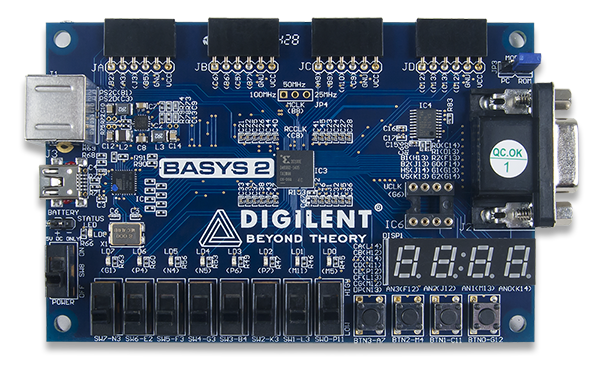
\includegraphics[width=\textwidth]{img/verilog/spartan3E-platine.png}
	\end{minipage}
	\begin{minipage}[b]{0.45\textwidth}
		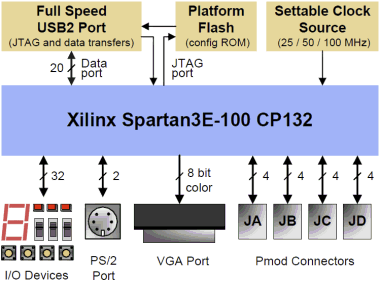
\includegraphics[width=\textwidth]{img/verilog/spartan3E-block.png}
	\end{minipage}

	\caption[Das Spartan-3E FPGA von Xilinx (links) mit entsprechendem Blockdiagramm (rechts).]{Das Spartan-3E FPGA von Xilinx\cite{basys2_board} (links) mit entsprechendem Blockdiagramm\cite{basys2_block} (rechts).\footnotemark}
	\label{fig:spartan3}

\end{figure}

\subsection{Einführung in Verilog}
Aus der 1983 vorgestellten Simulationssprache Verilog wurde 1990 durch den Aufkauf von Cadence Design Systems eine richtige Hardwarebeschreibungssprache. Über die Jahre hinweg wurde ausgelöst durch Kritik der Nutzer die Sprache immer weiter entwickelt. Der heutige Stand basiert auf einem 2002 verabschiedeten IEEE-Standard\cite{verilog_year}.

\subsubsection{Eigenschaften von Verilog}
\begin{itemize}
	\item klassischer HDL Workflow:
	\subitem \textbf{Synthese:} Erzeugen einer Netzliste aus der gegebenen Hardwarebeschreibung\cite{hdl_synthesis}
	\subitem \textbf{Simulation:} Testen der Schaltung bevor sie auf das FPGA geladen wird um Fehler zu entdecken, da Debugging auf der richtigen Hardware sehr schwer ist
	\subitem \textbf{Placing:} Basierend auf der Netzliste werden nun die entsprechenden Komponenten auf dem FPGA "`platziert"'
	\subitem \textbf{Routing:} Komponenten werden miteinander verbunden\cite{hdl_routing}
	\item Im Gegensatz zu normalen Programmiersprachen kann
	\textit{Gleichzeitigkeit} modelliert werden.
	\item Hochsprachenkonstrukte (and, or, if-else, \ldots)
	\item Modellierung auf \textit{Verhaltens-} und/oder
	\textit{Strukturebene} möglich
	\item Pfade können unterschiedlich lang sein und dadurch individuelle Verzögerung enthalten; auch die Logik selber hat eine individuelle Verzögerung. Daher muss auf den kritischen Pfad geachtet werden
\end{itemize}

\subsubsection{Modellierungsmethodiken}
\subsubsection*{Abstraktion}

Die Abstraktion erlaubt es, verschiedene Teile eines Modells
unterschiedlich detailliert zu beschreiben. Module, die nur für
die Simulation gebraucht werden, müssen z.~B. nicht so genau
beschrieben werden wie Module, die für die Synthese gedacht sind.

\noindent Die unterschiedlichen \textbf{Abstraktionsebenen} können folgendermaßen \textbf{grob eingeteilt} werden:
\begin{description}
	\item[Verhaltensbeschreibung:] Beschreibt lediglich funktionale Zusammenhänge. Dabei handelt es sich um algorithmische Beschreibungen mit den Mitteln einer höheren Programmiersprache,
	in der kein/kaum Bezug zur späteren Schaltungsstruktur genommen wird.
	
	\item[Datenflussbeschreibung:] Einfache logische Funktionen (AND, OR,
	NOT usw.) werden mit Verilog"--Sprachkonstrukten beschrieben,
	während komplexere Zusammenhänge durch Verwendung (meist vom
	Chiphersteller) vorgegebener Makrozellen erreicht werden. Ein Datenflussmodell
spiegelt viele Details der späteren Schaltung wieder.
	
	\item[Strukturbeschreibung:] Diese Art der Beschreibung stellt im
	Wesentlichen eine Netzliste der Schaltung dar. Hier werden alle
	Funktionen der Schaltung durch Verwendung (und Verschaltung) von
	Logikzellen beschrieben.
\end{description}

\subsubsection*{Modularität}
Die Modularität erlaubt es, große Funktionsblöcke zu unterteilen
und in abgeschlossene Unterblöcke, den sogenannten Modulen,
zusammenzufassen. Das erlaubt, den Funktionsblock besser zu
beherrschen ("`\textit{Teile und herrsche}"', engl. "`\textit{devide and conquer}"').



\subsubsection*{Hierarchie}
Die Hierarchie erlaubt es, ein System aus mehreren Modulen aufzubauen, die
wiederum aus mehreren Modulen bestehen können. Eine
Ebene in der Beschreibungshierarchie kann also ein oder mehrere
Module mit unterschiedlicher Abstraktion beinhalten. Die
Untermodule der darin enthaltenen Modulen bilden die nächste
darunterliegende Hierarchieebene.

\begin{itemize}
	\item Ein oder mehrere Module mit unterschiedlicher Abstraktion
	bilden eine Hierarchieebene. Die darin enthaltenen Untermodule
	bilden die Hierarchieebene darunter. 
	\item Teilbeschreibungen aus
	unteren Ebenen werden als Instanzen an übergeordnete Module
	weitergegeben.
\end{itemize}

Hierarchie bedeutet die Unterteilung der Gesamtschaltung in
einfachere und kleinere (Teil-) Komponenten. Diese sind
entsprechend der Struktur der Schaltung ineinander verschachtelt. Eine gegenseitige Verschachtelung ist freilich nicht erlaubt.\\
Die Komplexität dieser Komponenten kann von einem einzelnen
einfachen Gatter (z.~B. ein NAND) bis hin zu komplexen
Funktionseinheiten (z.~B. Prozessorkern, Filter usw.) reichen. Eine
Hierarchie stellt selber keine eigene Funktion innerhalb der
Schaltung dar, sondern kann als eine Hülle angesehen werden, in
der sich ein Schaltungsteil befindet. Die Hülle hat einen Namen
und verschiedene Anschlüsse zu der innen liegenden Schaltung,
deren Komplexität außerhalb verborgen bleibt und so eine
vereinfachte Betrachtung erst ermöglicht. Eine hierarchische
Struktur einer Schaltung lässt sich sehr leicht mit Koffern
vergleichen, die ineinander gelegt sind und in denen sich jeweils
ein Teil des Gesamt-Designs befindet. Die Gesamtschaltung kann man
dann mit dem obersten Koffer anfassen, da alle anderen sich in
diesem befinden.

\subsubsection{Komponenten der Verilog-Beschreibungssprache}
In Verilog wird zwischen \emph{Register} und \emph{Net} Datentypen unterschieden. Zusätzlich können \emph{konstante} Parameter in dem Datentyp \texttt{parameter} gepeichert werden \cite{IEEE_Verilog2001}. \\
Registertypen lassen sich unterteilen in:
\begin{itemize}
	\item \texttt{reg}. Werden meist für Ausgänge und speicherndes Verhalten verwendet. Sie können zu Bitarrays zusammengeschaltet sein und Signale treiben. Dieser Datentyp wird zur Logikbeschreibung verwendet.
	\item \texttt{integer}. Werden als Schleifenvariablen und Berechnungen zur Synthesezeit verwendet. Sie sind in der Regel 32 Bit breit.
	\item \texttt{time}. Ist ein vorzeichenloser 64 Bit Wert, welcher zur Speicherung von Zeiten in Testbenches geeignet ist.
	\item \texttt{realtime} und \texttt{real}. Fließkommazahlen mit doppelter Genauigkeit.
\end{itemize}
Die \emph{Net} Datentypen unterteilen sich in:
\begin{itemize}
	\item \texttt{wire}. Dienen zur Verbindung einzelner Module. Sie werden meist für Eingänge verwendet, können aber auch kombinatorische Logik durch beispielsweise \texttt{assign} realisieren. Wires können auch zur Umbenennung der Signale verwendet werden.
	\item \texttt{wor}, \texttt{wand}. Liefert eine kombinatorische \emph{OR} bzw. \emph{AND} Verknüpfung von mehreren \texttt{wire}.
	\item \texttt{supply0}, \texttt{supply1}. Liefert konstante 0 bzw. 1 mit hoher Treibfähigkeit. Dieser Typ sollte \textbf{nur} zur Definition der Versorgungs- und GND-Netzen verwendet werden.
\end{itemize}
Zusätzlich gibt es noch diverse Tri-State Net-Typen, die jedoch für das Praktikum irrelevant sind. Bei Interesse kann in der \emph{L}anguage \emph{R}eference \emph{M}anual (LRM) \cite{IEEE_Verilog2001} nachgelesen werden.\\
Zu beachten ist, dass nicht alle Datentypen für eine Synthese geeignet sind! So wird z.B. \texttt{time} und \emph{realtime} nur zu Simulationszwecke verwendet. Im Praktikum werden zusätzlich zu konstanten \texttt{parameter} der Typ \texttt{reg} und \emph{wire} für die Logikschaltung und Beschreibung verwendet.
\subsubsection*{Logikwerte}
Signale können vier verschiedene Werte annehmen:
\begin{table}[H]
	\begin{center}
		\begin{tabularx}{0.3\textwidth}{cl}
			\toprule
			\textbf{Name} & \textbf{Logikwert}\\
			\midrule
			\texttt{0} & logische Null\\
			\texttt{1} & logische Eins\\
			\texttt{X} & unbestimmt\\
			\texttt{Z} & hochohmig\\
			\bottomrule
		\end{tabularx}
		\caption{Logikwerte eines Signals}
	\end{center}
\end{table}
\texttt{0} und \texttt{1} sind klassische Logikwerte. \texttt{X} und \texttt{Z} sind jedoch hardwarespezifisch. Ersteres tritt auf, wenn ein Register keinen Wert zugewiesen bekommt und stellt nicht unbedingt einen Fehler dar. So lange ein Logikwert nicht verwendet wird, stellt \texttt{X} kein Problem dar und kann sogar die Synthesequalität verbessern. Besonders zum Debuggen lässt sich dies gut nutzen.\\
\texttt{Z} ist ein hochohmiger Zustand der dann auftritt, wenn zum Beispiel eine elektrische Verbindung getrennt werden soll.

Tabelle~\ref{tab:resolve} stellt dar, welches Endergebnis eine
Signalauswertung aus zwei Quellen erzeugen wird.
\begin{table}[h]
	\begin{center}
		\begin{tabularx}{0.2\textwidth}{ccccc}
			\toprule
			\textbf{\&}&\texttt{0}&\texttt{1}&\texttt{Z}&\texttt{X} \\
			\midrule
			\texttt{0}&\texttt{0}&\texttt{0}&\texttt{0}&\texttt{0}\\
			\texttt{1}&\texttt{0}&\texttt{1}&\texttt{X}&\texttt{X}\\
			\texttt{Z}&\texttt{0}&\texttt{X}&\texttt{X}&\texttt{X}\\
			\texttt{X}&\texttt{0}&\texttt{X}&\texttt{X}&\texttt{X}\\
			\bottomrule
		\end{tabularx}
		\caption{\texttt{AND}-Verknüpfung der Logikwerte}\label{tab:resolve}
	\end{center}
\end{table}

\begin{center}
	\noindent \fcolorbox{black}{white}{\parbox{0.95\textwidth}{
			Es muss immer darauf geachtet werden, dass
			\textbf{jedes Signal} immer nur \textbf{genau eine Quelle} hat. Insbesondere bedeutet das,
			dass ein Signal immer nur mit genau einem Ausgang genau einer
			Instanz verbunden sein darf oder dass ein Signal nur in genau
			einem \texttt{always} Block zugewiesen werden darf.\par
		}
	}
\end{center}

Eine Ausnahme von dieser Regel bilden Tristate-Signale. Solche
werden aber im Rahmen des Verilog-Teils dieses Praktikums nicht
verwendet.

\subsubsection*{Zahlen zuweisen und vergleichen}
Register können, genauso wie Variablen in Programmiersprachen, Werte zugewiesen bekommen. Dies ist bei der Definition der Variable immer mit einem normalen Gleichheitszeichen (\texttt{=}) und bei sequentieller Logik meist eine nicht blockierende Zuweisung (\texttt{<=}). Blockierende Zuweisungen haben den Nachteil, dass immer nur Zeile für Zeile nacheinander ausgeführt werden kann, genauso wie Software auf einem Mikroprozessor. Blockierende und Nichtblockierende Zuweisungen sollten nicht gleichzeitig in einem \texttt{always} Block verwendet werden.\\
Zu beachten ist jedoch der Fall, wenn der zugewiesene oder zu vergleichende Wert eine Zahl (z.B.: 45) ist. Eine einfache Zuweisung über \texttt{reg my\_register[5:0] = 45;} sollte vermieden werden. Stattdessen ist immer zu definieren, wie viele Bit breit und von welchem Zahlentyp die Zahl ist. \\
Die Bitbreite wird definiert über eine vorangehende Zahl (hier \texttt{6}) mit einem abschließenden Hochkomma. Darauf folgt die Definition des Zahlensystems (hier \texttt{d}). Hier gibt es die Optionen \textit{binär} (\texttt{b}), \textit{oktal} (\texttt{o}), \textit{dezimal} (\texttt{d}) und \textit{hexadezimal} (\texttt{h}).\\

\begin{figure}[h]
	%Hier beginnt der Quellcode
	\lstset{style=verilog-style}
	\lstinputlisting{verilog/numbers.v}
	%Hier endet der Quellcode
	\caption{Beispiel von verschieden Zahlen}
	\label{numbers}
\end{figure}

\subsubsection*{Module}
Alle Bestandteile der Verilog Beschreibung werden in einzelnen Modulen bearbeitet. Auch wenn es möglich ist, den ganzen Code in ein einziges Modul zu schreiben, ist es sinnvoll das Projekt in Untermodule zu unterteilen, wodurch Code auch mehrfach verwendet werden kann. 

\begin{figure}[h]
	%Hier beginnt der Quellcode
	\lstset{style=verilog-style}
	\lstinputlisting{verilog/module.v}
	%Hier endet der Quellcode
	\caption{Beispiel eines Modules mit Instantiierung eines Submodules}
	\label{module}
\end{figure}

In diesem Beispiel wird ein Module mit dem Namen \texttt{exModule} definiert. Nach dem Namen folgt die später noch erklärte Portliste, die in diesem Fall nur einen Eingang, die Clock, umfasst. Anschließend werden im Bereich unter der Portliste des Modules zwei \texttt{wire} definiert und ein Submodule instantiiert. \\
\texttt{exSubModule} ist in diesem Beispiel der Modulname, \texttt{exSubModule\_1} ist der Instanzname.

\subsubsection*{Portliste}
Die Portliste enthält die Schnittstellendefinition des Bausteins, die
sogenannten Ports. Bausteine kommunizieren miteinander über
Schnittstellen"=Signale.

Ein Port kann dabei eine einzelne Leitung oder eine Gruppe von
Leitungen (genannt Bus) beschreiben. Die Beschreibung des Signals auf einer
Leitung ist mit verschiedenen vordefinierten Typen möglich.

Ist kein Typ (\texttt{reg} oder \texttt{wire}) angegeben, so ist der Port immer vom Typ \texttt{wire} mit der Breite \texttt{1}.

\begin{figure}[H]
	%Hier beginnt der Quellcode
	\lstset{style=verilog-style}
	\lstinputlisting{verilog/portlist.v}
	%Hier endet der Quellcode
	\caption{Beispiel eines Modules mit Portliste}
	\label{portlist}
\end{figure}

\subsubsection*{Registerarrays und generische Breite}

Neben einfachen logischen Ein- und Ausgängen können in Verilog auch
Registerarrays (siehe Abb.~\ref{regarrays}) zum Einsatz kommen. Dies erleichtert die
Schreibarbeit bei großen Wörtern. \\
Außerdem ist es möglich ein Modul mit verschiedenen Parametern zu instantiieren, wodurch Codeduplikationen vermieden werden können.
\begin{figure}[H]
	%Hier beginnt der Quellcode
	\lstset{style=verilog-style}
	\lstinputlisting{verilog/addierzelle_entity_regarray.v}
	%Hier endet der Quellcode
	\caption{Beispiel einer Portliste mit Register-/Wirearrays}
	\label{regarrays}
\end{figure}
Die beiden Eingänge und der Ausgang sind damit 6 Bit breit. Diese Breite ist nun allerdings festgesetzt, so dass die Komponente nur eine Aufgabe für 6 Bit erfüllen kann. Oft ist es aber
nötig, das Komponenten innerhalb einer komplexen Beschreibung in
verschiedenen Breiten auftreten. Verilog bietet hier die Möglichkeit
einer generischen Wortbreite, die erst bei der Synthese der Komponente
deren Breite endgültig festlegt (siehe Abb. \ref{vektoren_generic}).
\begin{figure}[H]
	%Hier beginnt der Quellcode
	\lstset{style=verilog-style}
	\lstinputlisting{verilog/addierzelle_entity_generic.v}
	%Hier endet der Quellcode
	\caption{Registerarrays mit generischer Breite}
	\label{vektoren_generic}
\end{figure}


Diese Addierzelle hat nun eine generische Breite der Grundbreite
zehn aus dem Raum der natürlichen Zahlen. Wird das Modul verwendet, kann aber auch eine neue Breite über einen \texttt{parameter} angeben werden. Diese wird dann an die Registerarrays weitergeben. Ohne Angabe wird der Default-Wert (hier 10) benutzt. Wird kein Default"=Wert angegeben, muss beim Aufruf auf jeden Fall ein Wert für die Breite mitgegeben werden! \\
Außerdem kann \texttt{ADD1\_WIDTH} durch einen direkten Wert zu \texttt{Addierzelle \#(.WIDTH(6)) add1} geändert werden, falls auf einen \texttt{parameter} verzichtet werden soll.

\subsubsection*{Initial Block}
Gleich am Anfang nach der Definition der \texttt{reg} folgt der \texttt{initial begin} Block. Dieser wird nur einmalig zur Initialisierung des Modules ausgeführt und ist vergleichbar mit einem Klassenkonstruktor in C++. \\ \\
Dieser \texttt{initial begin} Block wird jedoch nicht zwingend in einem Modul benötigt, da einmalige Anweisungen auch so eingeführt werden, wenn sie sich im Modul befinden. Für eine Simulation ist hingegeben ist dieser Block sehr wichtig.

\begin{figure}[H]
	%Hier beginnt der Quellcode
	\lstset{style=verilog-style}
	\lstinputlisting{verilog/initial_begin.v}
	%Hier endet der Quellcode
	\caption{Beispiel eines Modules mit Initialisierung}
	\label{initial_begin}
\end{figure}

\subsubsection*{Always Block}
Im Hauptbereich des Moduls können \texttt{always} Blöcke verwendet werden um auf Signale bzw. deren Änderung zu reagieren. Nach der vollständiger Initialisierung können diese nun folgen. Ein solcher Always-Block kann auf eine positive Flanke (\texttt{posedge}), eine negative Flanke (\texttt{negedge}) oder eine generelle Änderung eines Signales reagieren. Diesen Bereich in den Klammern des \texttt{always} Blocks nennt sich \textit{Sensitivity List}.
\begin{figure}[H]
	%Hier beginnt der Quellcode
	\lstset{style=verilog-style}
	\lstinputlisting{verilog/always_posedge.v}
	%Hier endet der Quellcode
	\caption{Always Block, der auf eine positive Flanke der Clock reagiert}
	\label{always_posedge}
\end{figure}
\begin{figure}[H]
%Hier beginnt der Quellcode
\lstset{style=verilog-style}
\lstinputlisting{verilog/always_edge.v}
%Hier endet der Quellcode
\caption{Always Block, der auf jede Flanke der Clock reagiert}
\label{always_edge}
\end{figure}
Falls auf mehrere Signale reagiert werden soll, so können die Signale mit einem \texttt{or} verknüpft werden. In sequentiellen Design sollte nur auf eine Clockflanke reagiert werden, um die gewünschte Funktionalität der Logik zu realisieren.
\begin{figure}[H]
	%Hier beginnt der Quellcode
	\lstset{style=verilog-style}
	\lstinputlisting{verilog/always_multiple.v}
	%Hier endet der Quellcode
	\caption{Always Block, der auf mehrere Eingänge reagiert}
	\label{always_multiple}
\end{figure}
Des Weiteren gibt es noch die Signalliste von Verilog automatisch generieren zu lassen, indem man ein \texttt{*} verwendet. Das Synthesetool sucht sich nun selbst automatisch die Signale raus, auf die es reagieren soll. Diese Methode ist allerdings nicht empfohlen, da sie schnell zu ungewollten Fehlern führen kann.
\begin{figure}[H]
	%Hier beginnt der Quellcode
	\lstset{style=verilog-style}
	\lstinputlisting{verilog/always_star.v}
	%Hier endet der Quellcode
	\caption{Always Block, der automatisch auf Eingänge reagiert (hier jede Änderung von A oder B)}
	\label{always_star}
\end{figure}

Auch wenn hier in den Beispielen auf beliebige Signale reagiert wurde, sollte in der Anwendung darauf geachtet werden nur auf die Clock zu reagieren. Dies nennt sich dann sequentielle Logik. Es ist nicht sehr sauber und deutlich fehleranfälliger, wenn beispielsweise auf die positive Flanke eines Knopfdruckes reagiert wird. So ist beispielsweise in Abb. \ref{sens_1} und \ref{sens_2} zu erkennen, dass diese Konstrukte eine rein \emph{kombinatorische} generieren. Dabei ist zu beachten, dass \texttt{B} vom Typ \texttt{reg} ist, jedoch wird physikalisch \textbf{kein} Register verwendet.\\
Anders sieht es in Abb. \ref{sens_3} und \ref{sens_4} aus. Hier werden echte Register verwendet. Somit entsteht eine sequentielle Schaltung mit Speicher.

\begin{minipage}[H]{\textwidth}
	\begin{minipage}[H]{\textwidth}
		\begin{minipage}[b]{0.5\textwidth}
			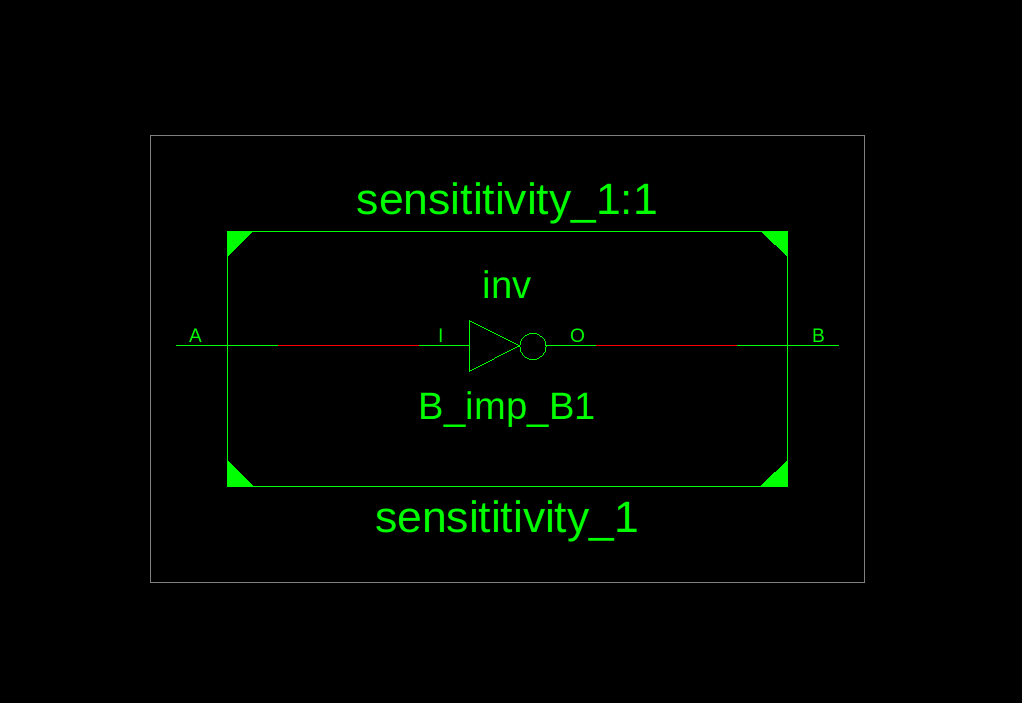
\includegraphics[width=\textwidth]{img/verilog/sens_1.png}
		\end{minipage}
		\begin{minipage}[b]{0.5\textwidth}
			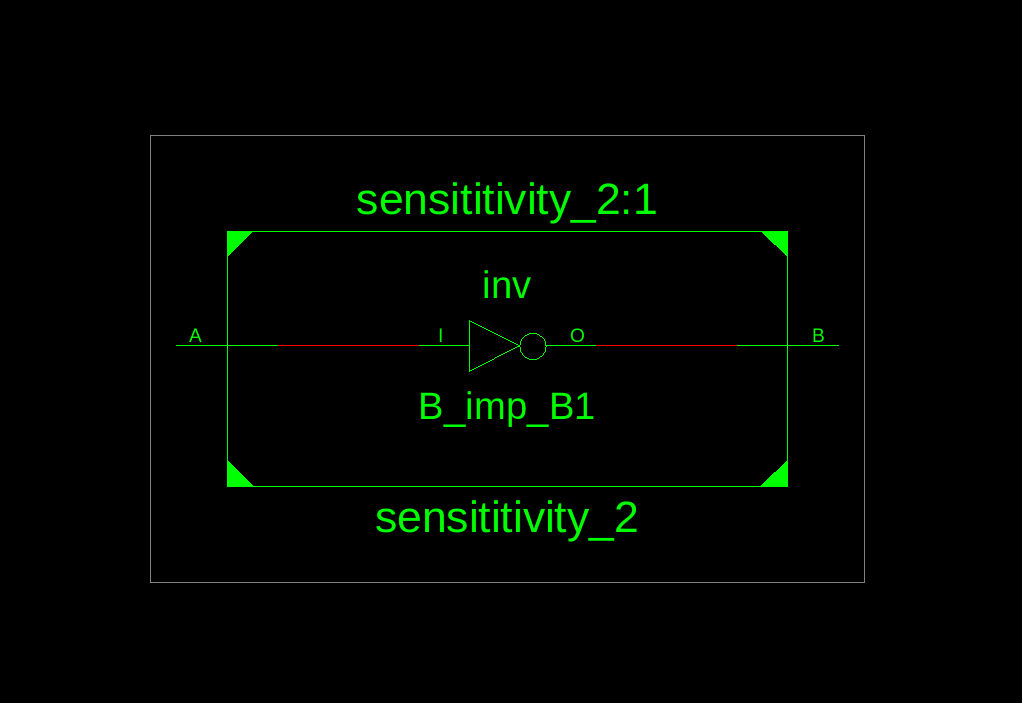
\includegraphics[width=\textwidth]{img/verilog/sens_2.png}
		\end{minipage}
	\end{minipage}
	\begin{minipage}[H]{\textwidth}
		\begin{minipage}[b]{0.5\textwidth}
			\centering
			\begin{minipage}[b]{0.9\textwidth}
				\begin{figure}[H]
					%Hier beginnt der Quellcode
					\lstset{style=verilog-style}
					\lstinputlisting{verilog/comp/sens_1.v}
					%Hier endet der Quellcode
					\caption{Reaktion auf jede Änderung} \label{sens_1}
				\end{figure}
			\end{minipage}
		\end{minipage}	
		\begin{minipage}[b]{0.5\textwidth}
			\centering
			\begin{minipage}[b]{0.9\textwidth}
				\begin{figure}[H]
					%Hier beginnt der Quellcode
					\lstset{style=verilog-style}
					\lstinputlisting{verilog/comp/sens_2.v}
					%Hier endet der Quellcode
					\caption{Reaktion auf jede Änderung von \texttt{A}} \label{sens_2}
				\end{figure}
			\end{minipage}
		\end{minipage}	
	\end{minipage}
	\\\\
	\hrule
	~\\\\
	\begin{minipage}[H]{\textwidth}
		\begin{minipage}[b]{0.5\textwidth}
			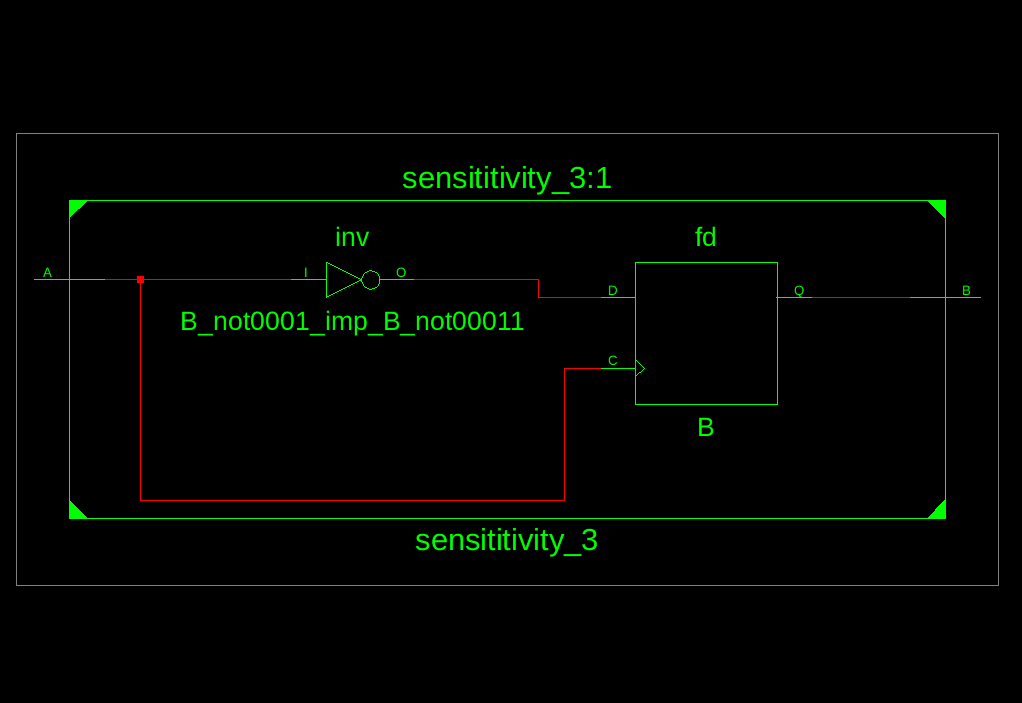
\includegraphics[width=\textwidth]{img/verilog/sens_3.png}
		\end{minipage}
		\begin{minipage}[b]{0.5\textwidth}
			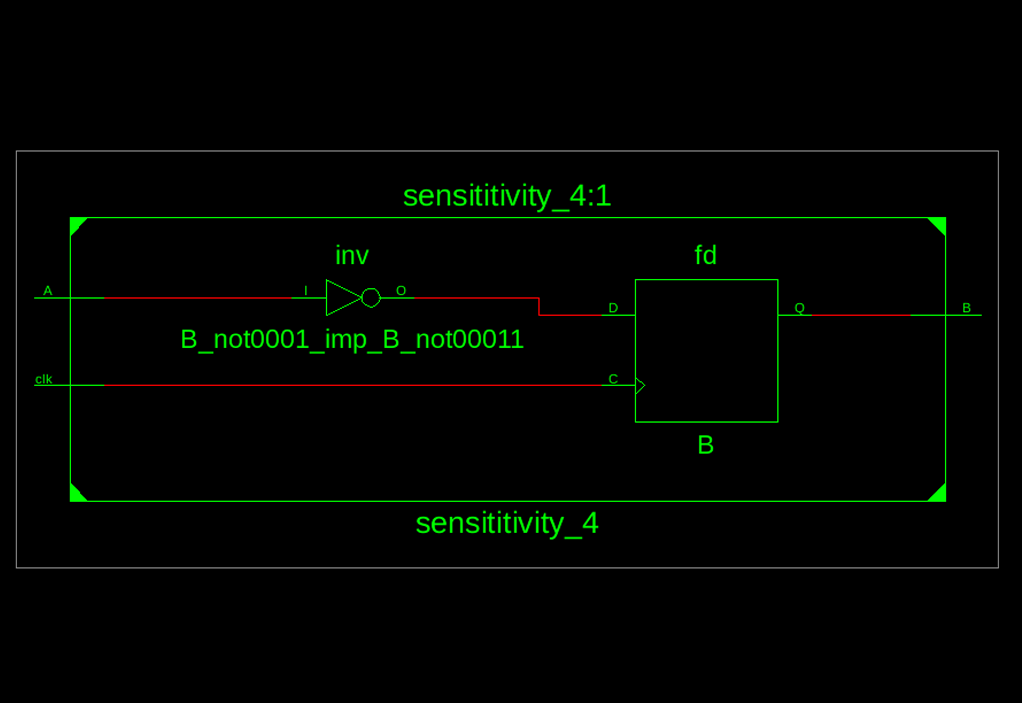
\includegraphics[width=\textwidth]{img/verilog/sens_4.png}
		\end{minipage}
	\end{minipage}
	\begin{minipage}[H]{\textwidth}
		\begin{minipage}[b]{0.5\textwidth}
			\centering
			\begin{minipage}[b]{0.9\textwidth}
				\begin{figure}[H]
					%Hier beginnt der Quellcode
					\lstset{style=verilog-style}
					\lstinputlisting{verilog/comp/sens_3.v}
					%Hier endet der Quellcode
					\caption{Reaktion auf \texttt{posedge A}} \label{sens_3}
				\end{figure}
			\end{minipage}
		\end{minipage}	
		\begin{minipage}[b]{0.5\textwidth}
			\centering
			\begin{minipage}[b]{0.9\textwidth}
				\begin{figure}[H]
					%Hier beginnt der Quellcode
					\lstset{style=verilog-style}
					\lstinputlisting{verilog/comp/sens_4.v}
					%Hier endet der Quellcode
					\caption{Reaktion auf eine Clock} \label{sens_4}
				\end{figure}
			\end{minipage}
		\end{minipage}	
	\end{minipage}
\end{minipage}
\\\\
Gut zu erkennen ist hier, wie kleine Änderungen der Sensitivitylist komplett andere Ergebnisse in den Logikschaltungen ergeben.\\
\begin{minipage}[H]{\textwidth} %force it into one block
	\begin{minipage}[H]{\textwidth}
		\begin{minipage}[H]{0.5\textwidth}
			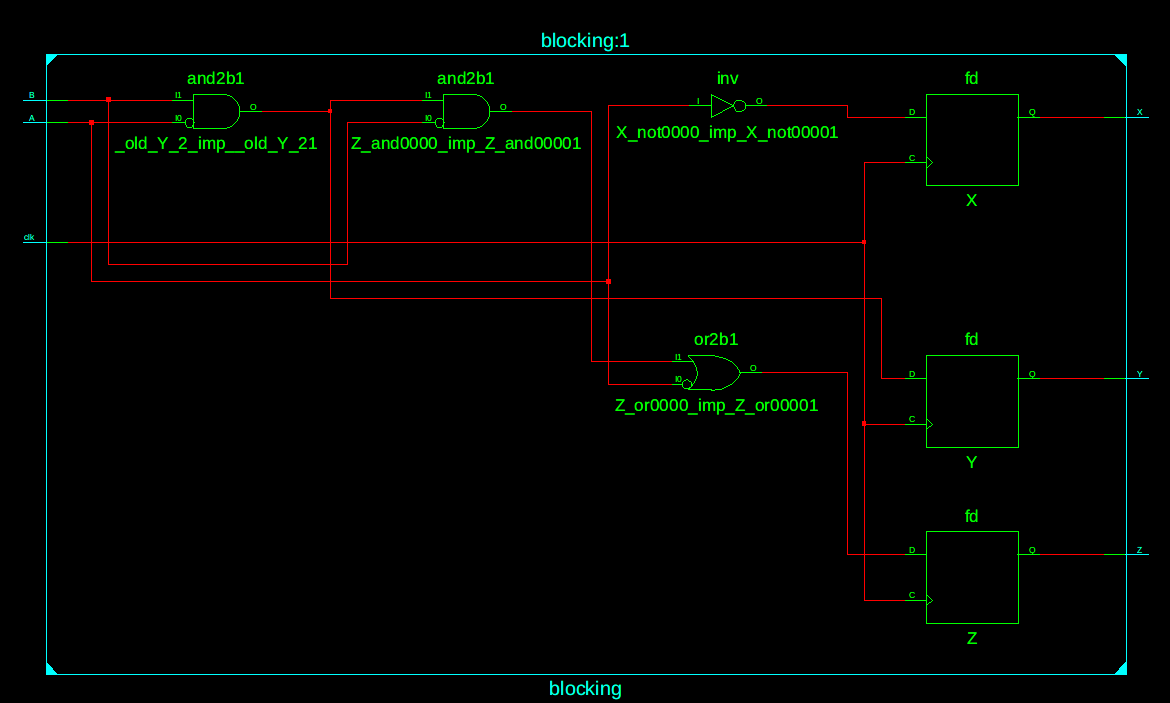
\includegraphics[width=\textwidth]{img/verilog/blocking.png}
		\end{minipage}
		\begin{minipage}[H]{0.5\textwidth}
			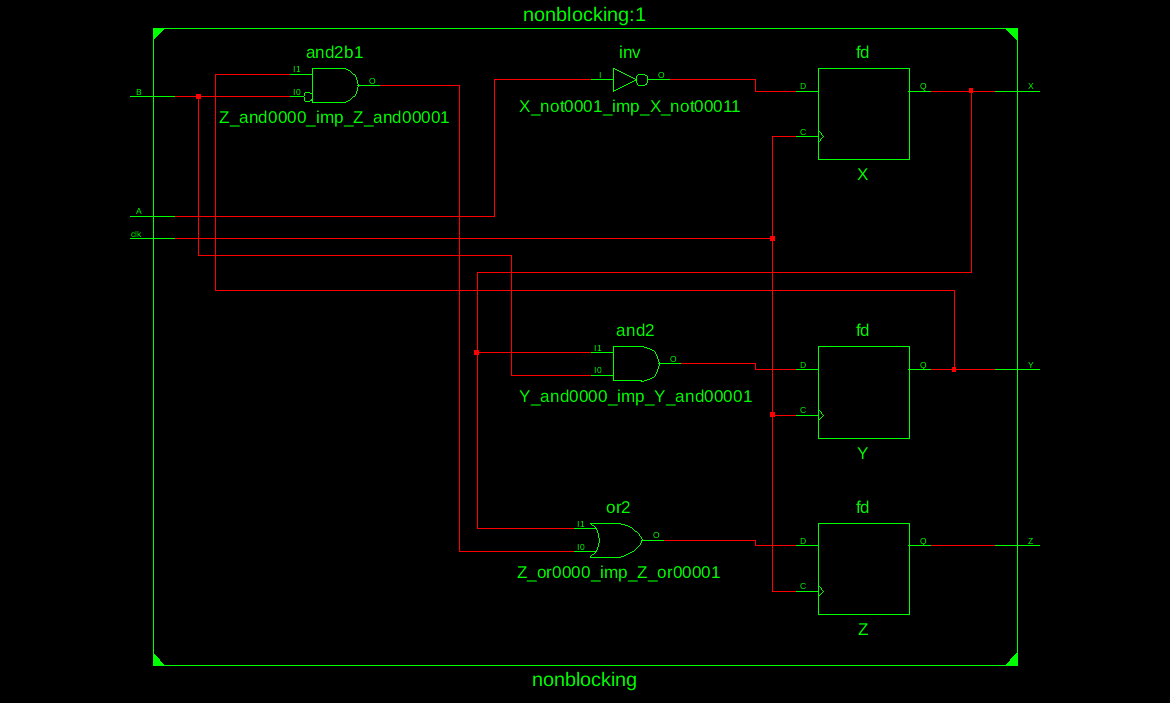
\includegraphics[width=\textwidth]{img/verilog/nonblocking.png}
		\end{minipage}
	\end{minipage}
	\begin{minipage}[H]{\textwidth}
		\begin{minipage}[H]{0.5\textwidth}
			\centering
			\begin{minipage}[H]{0.9\textwidth}
				\begin{figure}[H]
					%Hier beginnt der Quellcode
					\lstset{style=verilog-style}
					\lstinputlisting{verilog/comp/blocking.v}
					%Hier endet der Quellcode
					\caption{Blockierende Zuweisung} \label{blocking}
				\end{figure}
			\end{minipage}
		\end{minipage}	
		\begin{minipage}[H]{0.5\textwidth}
			\centering
			\begin{minipage}[H]{0.9\textwidth}
				\begin{figure}[H]
					%Hier beginnt der Quellcode
					\lstset{style=verilog-style}
					\lstinputlisting{verilog/comp/nonblocking.v}
					%Hier endet der Quellcode
					\caption{Nicht blockierende Zuweisung} \label{nonblocking}
				\end{figure}
			\end{minipage}
		\end{minipage}	
	\end{minipage}
\end{minipage}
\\\\
Im Vergleich zwischen blockierenden und nicht blockierenden Zuweisungen wird klar, warum in sequentieller Logik immer auf letzteres zurück gegriffen werden sollte. Diese Zuweisungen garantieren nämlich, dass beim Setzen eines Wertes alle benötigten Werte zur Verfügung stehen, da Ergebnisse in Flip-Flops zwischen gespeichert werden und damit Raceconditions verhindert werden können. Die nicht-blockierende Zuweisungen innerhalb eines Always-Blocks dienen dazu, \emph{parallele} Zuweisungen zu einem Zeitpunkt zu beschreiben.

\subsubsection{Sprachelemente}
Weitere wichtige Sprachelemente von Verilog ermöglichen die
Beschreibung von Schleifen und Abfragen.

\subsubsection*{If-Else}

Folgendes Code-Fragment benutzt eine \texttt{if}-Abfrage, um ein
Signal abhängig von einem anderen zuzuweisen:
\begin{figure}[H]
	%Hier beginnt der Quellcode
	\lstset{style=verilog-style}
	\lstinputlisting{verilog/if_else.v}
	%Hier endet der Quellcode
	\caption{If-Else Beispiel eines Multiplexers} \label{bspmuxif}
\end{figure}


Bei Synthese der entsprechenden Schaltung führen diese Zeilen (Abbildung~\ref{bspmuxif}) zur
Erzeugung eines Multiplexers. Es handelt sich um einen 2-zu-1 Multiplexer, dessen Wortbreite so groß wie die der {\em
mux\_}-Signale ist.  

Weiterhin ist darauf zu achten, das alle Zustände abgehandelt werden. Ansonsten wird ein Latch generiert, was im Digitaldesign unbedingt zu vermeiden ist. Alle \texttt{if} sollten nach Möglichkeit mit einem \texttt{else} abgeschlossen werden. 

\begin{minipage}[H]{\textwidth}
	\begin{minipage}[b]{0.5\textwidth}
		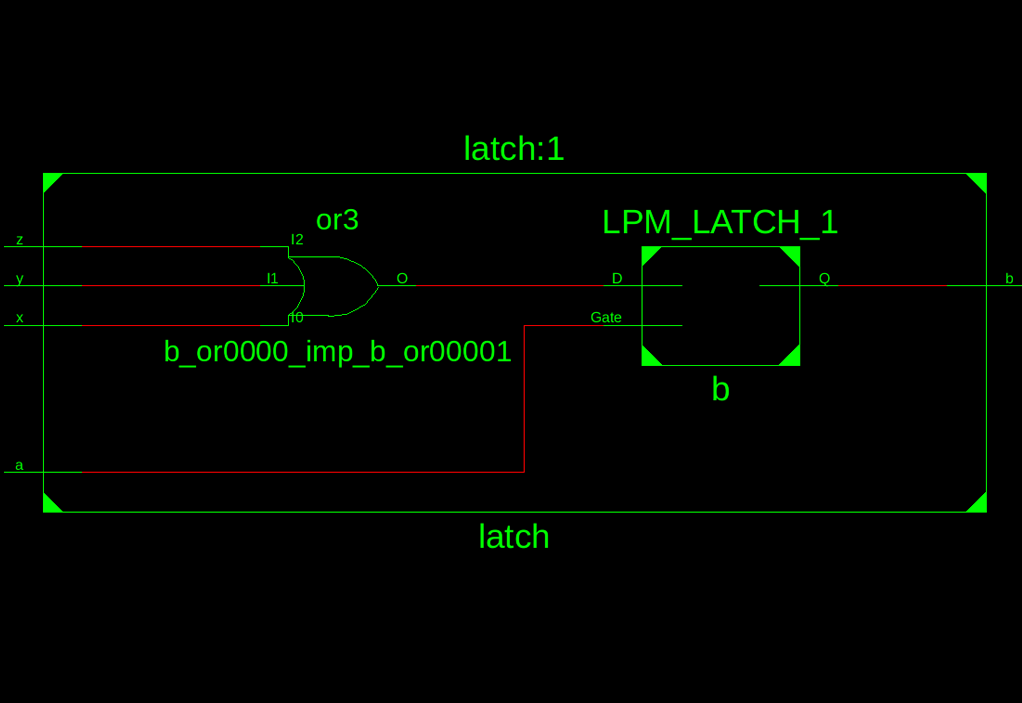
\includegraphics[width=\textwidth]{img/verilog/latch.png}
	\end{minipage}
	\begin{minipage}[b]{0.5\textwidth}
		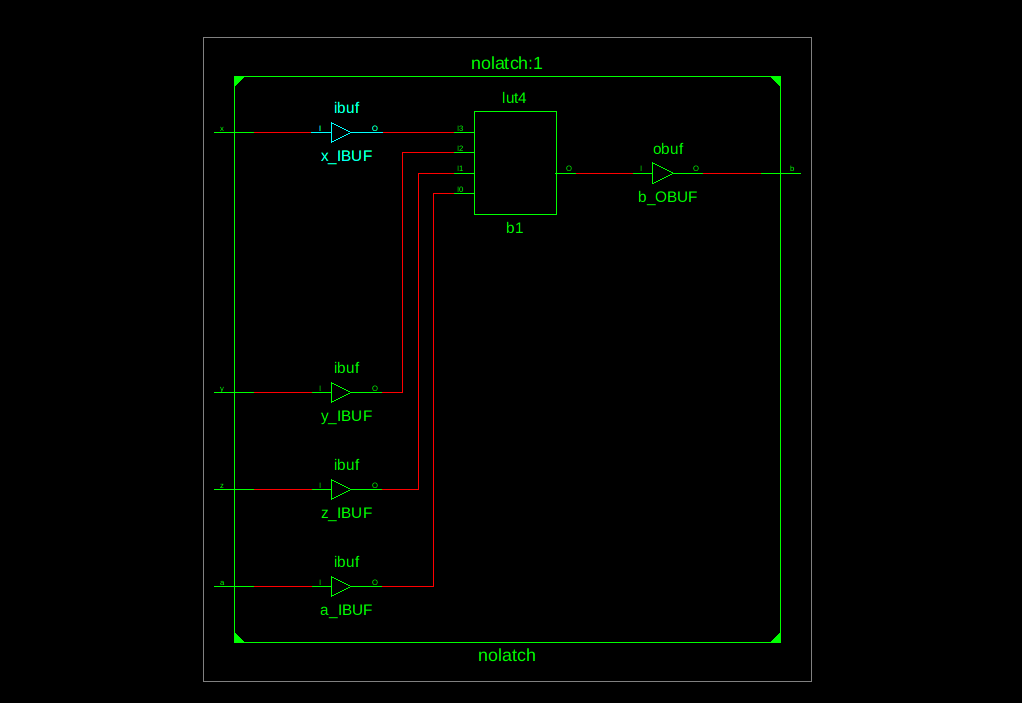
\includegraphics[width=\textwidth]{img/verilog/nolatch.png}
	\end{minipage}
\end{minipage}
\begin{minipage}[H]{\textwidth}
	\begin{minipage}[b]{0.5\textwidth}
		\centering
		\begin{minipage}[b]{0.9\textwidth}
			\begin{figure}[H]
				%Hier beginnt der Quellcode
				\lstset{style=verilog-style}
				\lstinputlisting{verilog/comp/latch.v}
				%Hier endet der Quellcode
				\caption{Beispiel eines ungewollten Latches} \label{bspinfif}
			\end{figure}
		\end{minipage}
	\end{minipage}	
	\begin{minipage}[b]{0.5\textwidth}
		\centering
		\begin{minipage}[b]{0.9\textwidth}
			\begin{figure}[H]
				%Hier beginnt der Quellcode
				\lstset{style=verilog-style}
				\lstinputlisting{verilog/comp/no_latch.v}
				%Hier endet der Quellcode
				\caption{Kein ungewolltes Latch} \label{bspnoinfif}
			\end{figure}
		\end{minipage}
	\end{minipage}	
\end{minipage}
\\\\

Dieses Latch entsteht, da der Ausgang dieser kombinatorischen Logik undefinierte Zustände hat (zB bei \texttt{a == 1'b0}) und damit den vorherigen Wert speichern muss. Jedoch hat kombinatorische Logik keine Flip-Flops und der Ausgang sollte immer direkt vom Eingang definiert werden. Der Synthetisierer muss daher einen Latch einbauen, um den fehlenden Zustand abzufangen. Dies führt, unter anderen auf Grund von Timingproblemen, zu fehlerhafter Hardware.

Außerdem sollte stets beachtet werden, dass die Tiefe der if-else Struktur nicht zu groß wird, da es zum Einen unübersichtlich wird und zum Anderen der kritische Pfad länger wird.

\subsubsection*{Case-Statement}

Eine andere Form der Abfrage, die diese Probleme nicht aufweist,
ist das \texttt{case}-Statement. Das Beispiel aus Abbildung~\ref{bspmuxif} könnte unter
Verwendung eines case-Statements folgendermaßen aussehen:

\begin{figure}[H]
	%Hier beginnt der Quellcode
	\lstset{style=verilog-style}
	\lstinputlisting{verilog/case.v}
	%Hier endet der Quellcode
	\caption{\texttt{case} Beispiel eines Multiplexers} \label{bspcase}
\end{figure}

Das \texttt{default}-Statement in dieser Beschreibung führt dazu,
dass der Ausgang auf \texttt{0} gesetzt wird, wenn \texttt{select} weder
\texttt{0} noch \texttt{1} ist.
\\\\
In folgenden Vergleich zwischen \texttt{if} und \texttt{case} ist zu erkennen, dass verschiedene Konstrukte zunächst unterschiedliche RTL-Logik generierten. \texttt{if-else-if} inferiert eine Vorrang-Logik, während \texttt{case} einen Multiplexer verwendet. \\
Die Abbildungen \ref{fig:bspif} und \ref{fig:bspswitch} zeigen jeweils \texttt{if} sowie \texttt{case} Konstrukte mit denen die resultierende Hardware aus Abbildung \ref{fig:if_vorrang} bzw. \ref{fig:case_multiplexer} beschrieben wird. Die Synthese der beiden Konstrukte für ein \emph{Xilinx Artix-7} FPGA ist jedoch identisch und in Abbildung \ref{fig:Synthese_FPGA_Artix_Case_If} dargestellt.

\begin{minipage}[H]{\textwidth}
	\begin{minipage}[b]{0.5\textwidth}
		\centering
		\begin{minipage}[b]{0.9\textwidth}
			\begin{figure}[H]
				%Hier beginnt der Quellcode
				\lstset{style=verilog-style}
				\lstinputlisting{verilog/comp/if_case.v}
				\caption{Beschreibung mit \texttt{if}} 
				\label{fig:bspif}
				%Hier endet der Quellcode

			\end{figure}
		\end{minipage}
	\end{minipage}	
	\begin{minipage}[b]{0.5\textwidth}
		\centering
		\begin{minipage}[b]{0.9\textwidth}
			\begin{figure}[H]
				%Hier beginnt der Quellcode
				\lstset{style=verilog-style}
				\lstinputlisting{verilog/comp/switch_case.v}
				\caption{Beschreibung mit \texttt{case}} 
				\label{fig:bspswitch}
				%Hier endet der Quellcode
			\end{figure}
		\end{minipage}
	\end{minipage}	
\end{minipage}

\begin{figure}[H]	
\frame{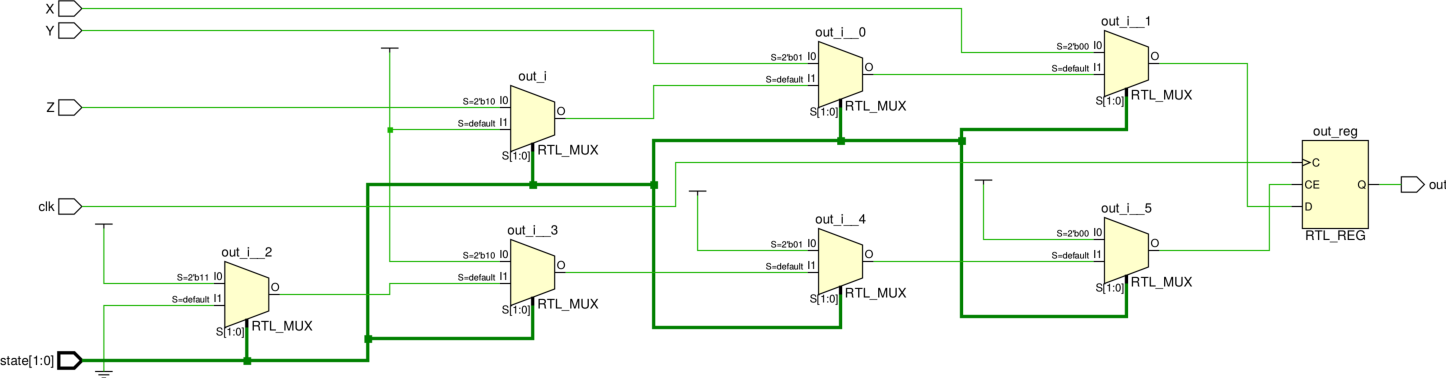
\includegraphics[width=\textwidth]{img/verilog/schematic_if_RTL}}
\caption{Vorrang-Logik mit \texttt{if}}
\label{fig:if_vorrang}
\end{figure}

\begin{figure}[H]	
\frame{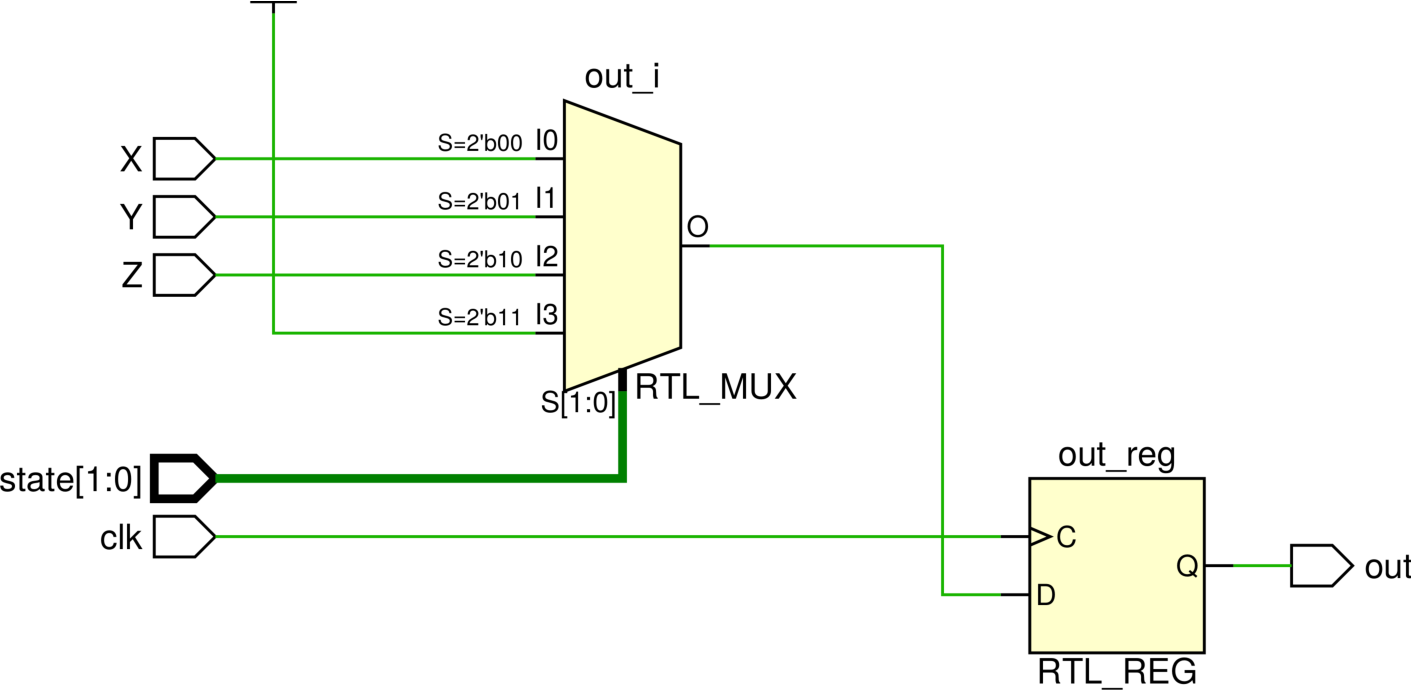
\includegraphics[width=\textwidth]{img/verilog/schematic_case_RTL}}
\caption{Multiplexer mit \texttt{case}} 
\label{fig:case_multiplexer}
\end{figure}


\begin{figure}[H]	
\frame{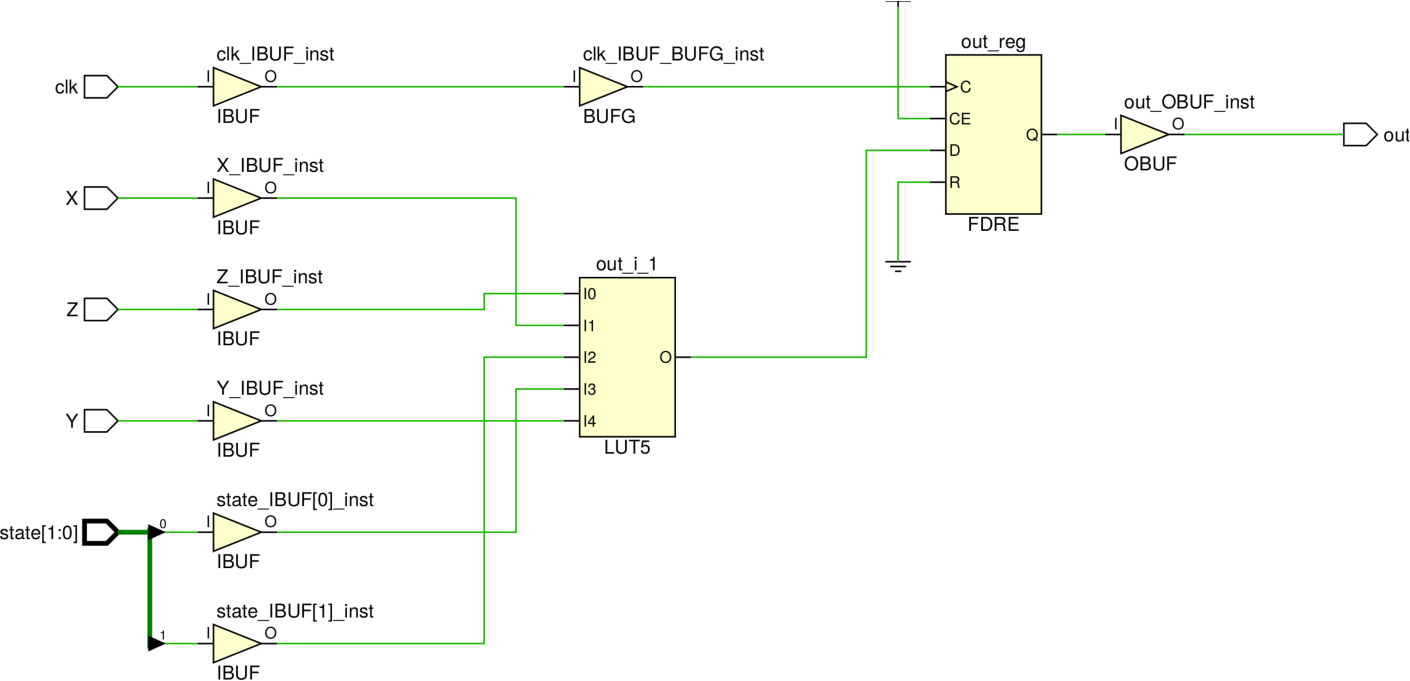
\includegraphics[width=\textwidth]{img/verilog/schematic_case_TECH}}
\caption[Synthese für ein Artix FPGA mit 5/6 Bit LUTs]{Resultierende Synthese für ein Artix FPGA mit 5/6 Bit LUTs der RTL-Logik aus obigen Abbildungen.} 
\label{fig:Synthese_FPGA_Artix_Case_If}
\end{figure}

\subsubsection*{Schleifen}
Eine aus den klassischen Programmiersprachen bekannte Schleife gibt es in Verilog nicht, aber es gibt dennoch zwei Dinge, die unter diesen Überbegriff passen. \textbf{Macro Loops} und \textbf{Custom Loops} (der Name wird hier definiert als Beschreibung einer Loop, die in einem \texttt{always} Block geschrieben wird).

Die sogenannten \textbf{Macro Loops} sind Schleifen, die vor der Synthese ausgeführt werden und automatisch Code erzeugen. Daher eignen sie sich sehr gut um sich wiederholende Strukturen zu vereinfachen.

\begin{figure}[h]
	%Hier beginnt der Quellcode
	\lstset{style=verilog-style}
	\lstinputlisting{verilog/generate_loop.v}
	%Hier endet der Quellcode
	\caption{\texttt{For Loop} in einem \texttt{generate} Block} \label{bspgenloop}
\end{figure}

Der Code in diesem Beispiel instantiiert acht Mal das Multiplexermodul aus vorherigen Beispielen. Dabei haben wir eine \texttt{genvar index}, die den Index der Schleife hoch zählt und sich dafür nutzen lässt bestimmte einzelne Signale aus einem Array abzugreifen. \\
Diese Art der Schleife kann in jeder beliebigen Situation genutzt werden. Ein Beispiel wäre die Ansteuerung mehrerer LEDs. Der \texttt{generate} Block würde dann sozusagen den Code für die Ansteuerung aller LEDs untereinander schreiben und kann somit natürlich auch in einem \texttt{always} Block verwendet werden. \\
Soll aber Hardware gespart werden, dann eignet sich eine \textbf{Custom Loop}. Eine Schleife in einem \texttt{always} Block, die bei jedem Clock-Zyklus eine weitere Aktion ausführt.

\begin{figure}[h]
	%Hier beginnt der Quellcode
	\lstset{style=verilog-style}
	\lstinputlisting{verilog/always_loop.v}
	%Hier endet der Quellcode
	\caption{Eine auf mehrere Takte verteilte ``Schleife''.} \label{bspalwloop}
\end{figure}
Zusätzlich gibt es die Möglichkeit mit Hilfe einer \texttt{FOR} Schleife innerhalb eines Always-Blocks Codezeilen zu sparen. Diese Schleife wird \emph{entfaltet} und generiert die gewünschte Hardware. Ein Beispiel eines langen Schieberegisters ist in der Abbildung \ref{vektoren_generic} dargestellt.
\begin{figure}[H]
	%Hier beginnt der Quellcode
	\lstset{style=verilog-style}
	\lstinputlisting{verilog/for_loop_always.v}
	%Hier endet der Quellcode
	\caption{\texttt{FOR} Schleife in einem \texttt{always} Block zur Erzeugung eines Schieberegisters} \label{bspforloop_always}
\end{figure}
\subsubsection*{Operatoren und Zuweisungen}

Verilog kennt unter anderem folgende relationale Operatoren:
\begin{align*}
==& \quad \text{gleich} \\
===& \quad \text{Fallgleichheit (X und Z werden auch verglichen)}\\
!=& \quad \text{ungleich} \\
<& \quad \text{kleiner als} \\
<=& \quad \text{kleiner gleich} \\
>& \quad \text{größer} \\
>=& \quad \text{größer gleich} 
\end{align*}

Bei Zuweisungen werden folgende Symbole verwendet:
\begin{align*}
=& \quad \text{Variablenzuweisung, bzw. blockierende Signalzuweisung} \\
<=& \quad \text{nicht blockierende Signalzuweisung} 
\end{align*}

Die bekannten logischen Operatoren sind hier auch verfügbar:
\begin{align*}
!& \quad \text{logische \texttt{Negation}} \\
||& \quad \text{logisches \texttt{oder}} \\
\&\&& \quad \text{logisches \texttt{und}}
\end{align*}

Ebenso die bitweisen Operatoren:
\begin{align*}
\sim& \quad \text{Negation} \\
\&& \quad \text{und}\\
|& \quad \text{oder (inklusiv)} \\
\hat{}& \quad \text{oder (exklusiv)}
\end{align*}

Dies ist lediglich ein Auszug. Natürlich können zum Beispiel auch "`$+$"'~und~"`$-$"' verwendet werden. Der Synhetisierer erkennt aus dem Kontext, ob es sich um eine
Signalzuweisung oder einen Vergleich kleiner/gleich handelt. Außerdem können Bits in einem \texttt{reg} mittels \textit{Bitshifting} (\texttt{>{}>} und \texttt{<{}<}) verschoben werden.

\subsubsection{Beschreibung sequentieller Schaltungen in Verilog}
Bisher haben wir in Verilog nur die M\"{o}glichkeit, kombinatorische
Schaltungen zu beschreiben. Für eine Ansteuerung, wie wir sie
implementieren wollen, wird das mit Sicherheit nicht ausreichend
sein, da auch sequentielle Schaltungsteile (z.B. Flip-Flops und
Register) in solchen Schaltungen vorkommen.

Gl\"{u}cklicherweise lassen sich solche sequentiellen Elemente in
Verilog mit den bisher betrachteten Sprachelementen bereits
beschreiben. Wir haben schon im vorangehenden Kapitel gesehen, 
dass mit einem einfachen \texttt{if}-Befehl
bereits die Beschreibung eines Latches m\"{o}glich ist. Ein solches
Latch ist bereits ein speicherndes Element, d.h. ein Teil einer
sequentiellen Schaltung.

Betrachten Sie das Beispiel eines Latches in Abb.~\ref{latch}.
\begin{figure}[h]
	%Hier beginnt der Quellcode
	\lstset{style=verilog-style}
	\lstinputlisting{verilog/d_latch.v}
	%Hier endet der Quellcode
	\caption{Verilog-Beschreibung eines D-Latch}
	\label{latch}
\end{figure}


Unser \texttt{always}-Block ist immer dann aktiv, wenn sich \texttt{D}
oder \texttt{L} \"{a}ndern. Dabei wird jedesmal, wenn \texttt{L=1} ist, \texttt{D} an den
Ausgang \texttt{Q} weitergereicht. Dies bedeutet, dass jede \"{A}nderung von \texttt{D} auch am Ausgang \texttt{Q} sichtbar ist, solange \texttt{L=1} ist. Es wird gesagt:
Das Latch ist transparent bei \texttt{L=1}. 

\"{A}ndert sich \texttt{D} jedoch,
w\"{a}hrend \texttt{L=0} ist, so wird diese \"{A}nderung nicht
weitergereicht. Mit anderen Worten: Der Ausgang \texttt{Q} \"{a}ndert sich
nicht. Er kann daher logischerweise nur auf seinem vorherigen Wert
bleiben.

Da der Ausgang \texttt{Q} abh\"{a}ngig ist vom Zustand des Eingangs \texttt{L}, ist ein
Latch immer \textbf{pegelgesteuert}.


Leider sind solche Latches -- wegen der Transparenz w\"{a}hrend
\texttt{L=1} und der Pegelsteuerung -- nur bedingt f\"{u}r den Aufbau
sequentieller Schaltungen geeignet. Allerdings kann (wie in der
Vorlesung Mikroelektronik 1 vorgestellt) aus zwei
pegelgesteuerten Latches ein \textbf{flankengesteuertes}
Flip-Flop aufgebaut werden.

Flip-Flops k\"{o}nnen jedoch auch (ebenfalls in Mikroelektronik 1
beschrieben) aus r\"{u}ckgekoppelten Gattern (z.B. NAND) aufgebaut
werden.

In Verilog ist es allerdings nicht erforderlich, ein Flip-Flop unter
der Verwendung solcher Latches oder r\"{u}ckgekoppelter Gatter zu
beschreiben. Mit einem \texttt{always} Block kann n\"{a}mlich
in einer Verilog-Beschreibung auf die \emph{\"{A}nderung eines
	Signals}, d.h. auf eine \emph{Flanke}, reagiert werden (siehe Abb.~\ref{dff}).
\begin{figure}[H]
	%Hier beginnt der Quellcode
	\lstset{style=verilog-style}
	\lstinputlisting{verilog/d_flip_flop.v}
	%Hier endet der Quellcode
	\caption{D-Flip-Flop in Verilog}
	\label{dff}
\end{figure}

Da ein \textbf{flankengesteuertes} Element (z.B. mit dem Signal
\texttt{clk}) nur bei der entsprechenden Flanke aktiv wird,
besteht die Sensitivity List ebenfalls nur aus diesem einen Signal.

Das so beschriebene D-Flip-Flop ist eine rein synchrone Schaltung.
Ein Flip-Flop mit asynchronem Reset kann daraus sehr einfach
gewonnen werden. Dabei muss jedoch beachtet werden, dass das
Flip-Flop nun nicht mehr nur von der Taktflanke, sondern auch vom
Reset-Signal aktiviert werden kann, d.h. dass das Reset-Signal
ebenfalls in die Sensitivity List aufgenommen werden muss (siehe Abb.~\ref{dff_asreset}).
\begin{figure}[H]
	%Hier beginnt der Quellcode
	\lstset{style=verilog-style}
	\lstinputlisting{verilog/d_flip_flop_as.v}
	%Hier endet der Quellcode
	\caption{D-Flip-Flops mit asynchronem Reset}
	\label{dff_asreset}
\end{figure}
Bei einem Flip-Flop mit synchronem Reset dagegen wird das
Reset-Signal nur dann ausgewertet, wenn eine steigende
Taktflanke anliegt (siehe Abb.~\ref{dff_sreset}).

\begin{figure}[H]
	%Hier beginnt der Quellcode
	\lstset{style=verilog-style}
	\lstinputlisting{verilog/d_flip_flop_s.v}
	%Hier endet der Quellcode
	\caption{D-Flip-Flops mit synchronem Reset}
	\label{dff_sreset}
\end{figure}


Aus Flip-Flops lassen sich Register realisieren, die mehrere Bits gleichzeitig speichern können. Wenn wir uns die Beschreibung der Flip-Flops etwas genauer ansehen, erkennen wir, dass die Breite von \texttt{Q} und \texttt{D} in den Beispielen \texttt{1} ist. D.h. es wird genau ein Flip-Flop instanziiert. Die Breite kann jedoch erhöht werden. Dadurch werden mehrere Flip-Flops als ein Register genutzt. Die Grundlagen dazu wurden in \emph{Mikroelektronik 1/2} behandelt.

\begin{center}
\noindent\fcolorbox{black}{white}{\parbox{0.95\textwidth}{
Standardmäßig werden in Verilog die Werte eines Registerarrays mit einer einfachen Zuweisung wie \texttt{reg my\_reg[5:0] = 6'b0} gesetzt um alle sechs Bits auf Null zu setzen. \\
Es lässt sich aber auch kombinieren aus einzelnen Teilen mit \texttt{\{\}} Klammern. Beispielsweise setzt \texttt{reg my\_reg[5:0] = \{4'b1, 2'b0\}} die ersten vier Bits auf eins, die letzten beiden auf null. Dies wird auch \textbf{Konkatenation} genannt.\\
Das Zusammenfügen lässt sich sogar noch mit Faktoren erweitern. Um das gleiche Ergebnis wie zuvor zu erhalten, lautet die Zeile daher \texttt{reg my\_reg[5:0] = \{4\{1'b1\}, 2\{1'b0\}\}}. \texttt{\{4\{1'b1\}\}} wird als \textbf{Replikation} bezeichnet.
}}
\end{center}

\subsubsection{Pipelining}\label{subsec:pipelining}
\emph{Pipelining} hat das Ziel, die benötigte Zeit für sequentielle Berechnungen zu reduzieren. In Hardware entspricht die Zeit einer Anzahl an Clock-Zyklen, welche für eine Berechnung benötigt werden. In Abbildung \ref{fig:pipeline} wird das Prinzip des Pipelining dargestellt.
Unter der Annahme, dass ein Modul \texttt{FOO} \mbox{$ k=5 $} Takte (A  \textasciitilde\, E) benötigt, um eine Berechnung durchzuführen und diese Berechnung für verschiedene Eingangswerte $ m=4 $ mal durchgeführt werden soll, ergibt sich eine Dauer von $ k\cdot m = 20 $ Takten. In diesem Fall werden 5 Takte für die Berechnung benötigt. In der Berechnungszeit werden also keine neuen Werte angenommen. Es muss folglich gewartet werden, bis die Berechnung durchgeführt wurde. In manchen Designs bzw. Modulen wird aber aus verschiedenen Gründen ein hoher Durchsatz (Verarbeitungsgeschwindigkeit) gefordert. Beispielsweise wenn auf einer Pixelpipeline gearbeitet wird, die mit der entsprechenden Pixelclock getaktet ist (siehe Kapitel \ref{subsec:display_timing}). \\
Um dieses Problem zu lösen kann das obige Modul \texttt{FOO} so erweitert werden, dass eine sog. Pipeline ermöglicht wird. Dazu werden jedoch zusätzliche Register im Modul nötig. In diesen werden die jeweiligen Zwischenergebnisse der einzelnen \emph{Stufen} gespeichert. Wird dieses Modul so implementiert, dass es in \textbf{jedem} Takt einen neuen Wert einliest und nach einer einmaligen Vorlaufzeit von 5 Takten, jeden Takt das nächste Ergebnis liefert, wird für dieses Beispiel mit 4 nacheinander folgenden Werten eine \emph{Geschwindigkeitsgewinn} von 2,5 erreicht. Diese kann für eine $k $-stufige Pipeline und $ m $ sequentiellen Werten berechnet werden zu \cite[p.286]{molitor}:
\begin{equation}
\mathrm{speedup} = \frac{k\cdot m}{k+ (m-1)}
\end{equation}
Beispielsweise sollen $ 1920 \cdot 1080$ Werte ($ N $-Bit) nacheinander mit einer $ N $-Bit Zahl multipliziert werden. Ohne Pipelining benötigt die Berechnung jeweils $ N+1 $ Takte. Insgesamt $ 1920 \cdot 1080 \cdot (N+1) $ Takte. Wird ein Multiplizierer mit Pipelining verwendet, werden hingegen nur $ 1920 \cdot 1080 + N $ Takte benötigt. Der Geschwindigkeitsgewinn nähert sich also $ N $, für $ m \gg k $.
\begin{figure}[H]
	\centering
	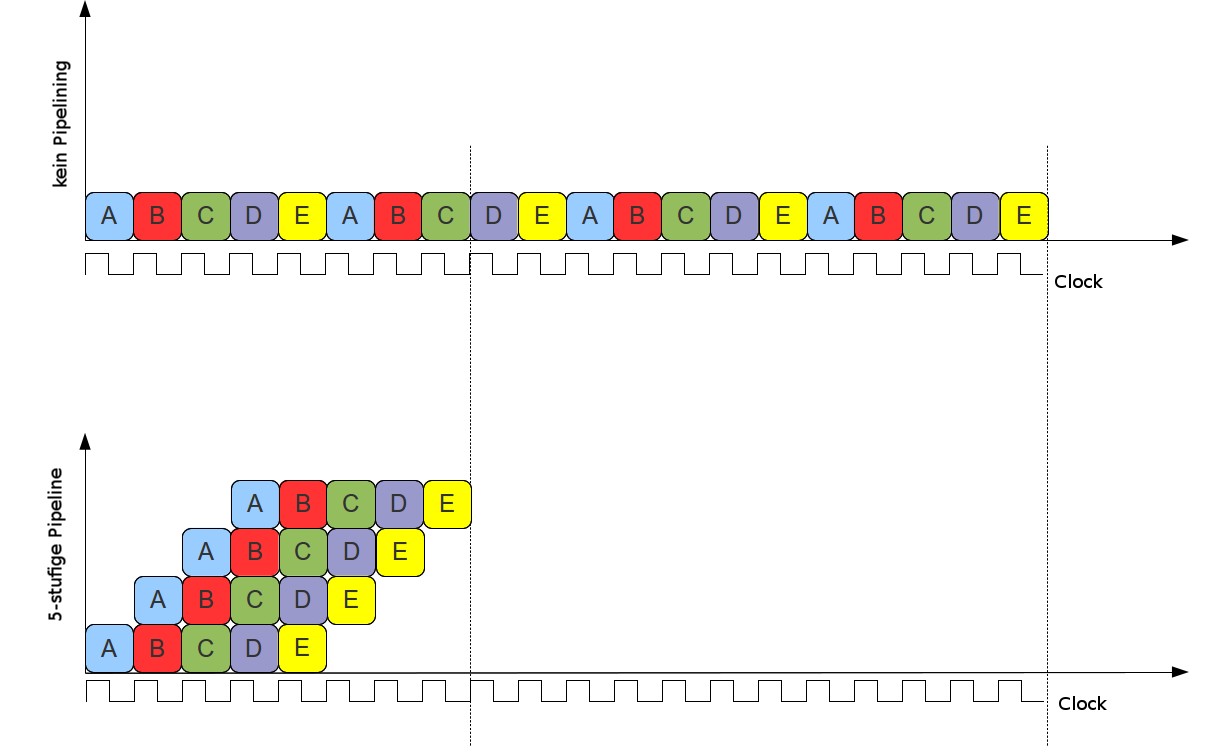
\includegraphics[width=\linewidth]{img/verilog/pipelining.png}
	\caption[Funktionsprinzip von Pipelining]{Funktionsprinzip von Pipelining. Oben Ausführung ohne Pipeline. Unten Implementierung mit Pipelining. Entnommen aus \cite{Derjavitch2012}.}
	\label{fig:pipeline}
\end{figure}

\pagebreak

\subsection{Xilinx ISE}
ISE ist eine Entwicklungsumgebebung (IDE) der Firma Xilinx zum Schreiben und Testen von Verilog Hardware-Designs.

\subsubsection{Neues Projekt}
Zuerst muss ein neues Projekt mit denen in Abb. \ref{fig:new_project} gezeigten Werten erstellt werden. Anschließend erscheint im \texttt{Hierarchy} Fenster eine FPGA-Bezeichnung. Eine neue Sourcedatei kann im Kontextmenü dieses Elementes erzeugt werden. Hierfür wählt man den Typ \texttt{Verilog Module} aus.\\
Weitere Sourcedateien können an beliebiger Stelle im Baum erzeugt werden, sie werden automatisch nach dem Einbinden im Code automatisch eingeordnet.

\begin{figure}[H]
	\centering
	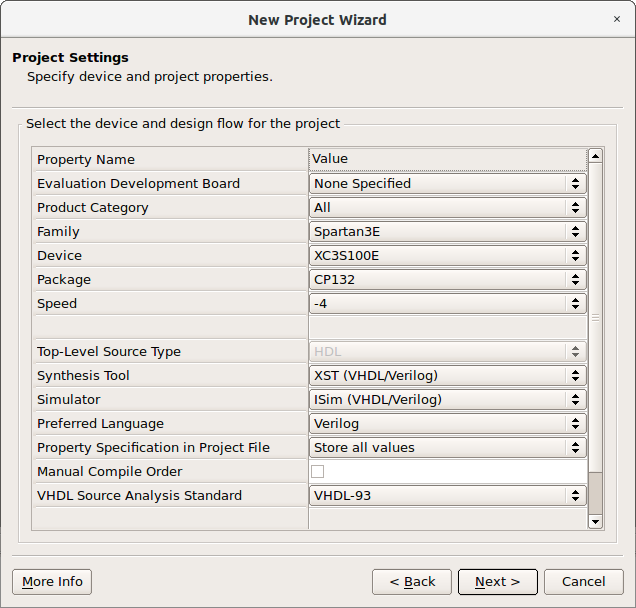
\includegraphics[width=0.55\linewidth]{img/verilog/new_project.png}
	\caption{Einstellungen für ein neues Projekt}
	\label{fig:new_project}
\end{figure}

\subsubsection{Testbench / Simulation}
Es empfiehlt sich den Code zu testen, bevor er auf das Board geladen wird, da das Debuggen von Hardware oftmals nur mit sehr großem Aufwand möglich ist. Für kleine Tests eignen sich beispielsweise vorhandene LEDs oder Pins.\\
Hierfür erstellt man auch wieder eine neue Verilog Source Datei. Es empfiehlt sich hier die vordefinierte Datei \texttt{Verilog Test Fixture} zu verwenden, da so alle kritischen Strukturen bereits gegeben sind. Außerdem muss diese Datei noch aus dem Sourcebaum genommen werden. Einstellungen dafür findet man im Kontextmenü unter \texttt{Source Properties ...} > \texttt{Design View} > \texttt{View Association} > \texttt{Simulation}. \\
Wenn man nun \texttt{Simulate Behavioral Model} in der \texttt{Simulation} Ansicht doppelklickt öffnet sich die Testbench.
\\ \\
Wie in dem Beispiel in \ref{testbench} zu sehen, besteht eine solche Testbench aus den gleichen Elementen wie auch eine normale Verilog Hardware. \\
Nach der Definition der zeitlichen Auflösung, wird das Testmodul (ohne Portliste) definiert. Alle Ein- und Ausgänge des anschließend instantiierten Hauptmoduls, die normalerweise über die Constraintsdatei mit der IO verknüpft sind, werden in dieser Testbench simuliert. \\
Es gibt einen \texttt{initial begin} Block, in dem die Variablen alle initialisiert werden und einmal auszuführende Schritte definiert werden. Es ist wichtig die Testwerte erst nach einer Pause zu starten, da das Setup der Hardware einen Moment dauert. \\
Außerdem können beliebig viele \texttt{always} Blöcke eingefügt werden, die unabhängig voneinander Signale immer wieder ändern. Hier am Beispiel einer Clock, die natürlich auch generiert werden muss. \\
Pausen sind abhängig von der ersten der beiden Zahlen hinter dem \texttt{'timescale} Befehl und beginnen immer mit \texttt{\#}. \\
Dieser \texttt{'timescale} Befehl hat zwei Argumente, wovon die erste der beiden Zahlen die Zeitauflösung (\emph{time\_unit}) angibt. Die Zweite Zahl definiert die Präzision (\emph{time\_precision}). Lautet also die Zeile \texttt{'timescale 1ns/1ns}, so ist die Zeitauflösung \texttt{1\,ns} und die Präzision \texttt{1\,ns}, also existieren keine Nachkommastellen. In Abb. \ref{testbench} gibt es daher drei Nachkommastellen. Erlaubte Werte sind jeweils 1,10 und 100 mit den Einheiten \texttt{s, ms, us, ns, ps} sowie \texttt{fs}.\\
Die resultieren Delay Zeit hinter einem \texttt{\#} berechnet sich also zu 
\begin{equation*}
\mathrm{t_{temp}} = \#\mathrm{X} \cdot {time\_unit}
\end{equation*}
$ t_{temp} $ wird schließlich zum nächsten Integer-Vielfachen der \emph{time\_precision} aufgerundet. So ergibt beispielsweise eine \texttt{'timescale 10ns/10ns} für ein Delay $ \texttt{\#1.5} $ eine Zeit von 20\,ns.

\begin{figure}[H]
	%Hier beginnt der Quellcode
	\lstset{style=verilog-style}
	\lstinputlisting{verilog/testbench.v}
	%Hier endet der Quellcode
	\caption{Beispiel einer Testbench}
	\label{testbench}
\end{figure} 

\subsubsection{Spezifizierung von Constraints}
Neben den Verilog Dateien hat jedes ISE-Projekt auch eine \texttt{*.ucf}-Datei, in der die Constraints beschrieben werden. In dieser werden unter anderem die Ports des Top-Moduls mit den Pins des FPGA verbunden (\texttt{LOC} constraints). Die Angaben dazu findet man in dem Datenblatt des FPGAs. Zusätzlich werden Frequenzen, Delays usw. der verschiedenen verwendeten Clocks spezifiziert. Dadurch kann beim Placing und Routing auf den \emph{kritischen Pfad} geachtet werden.

\begin{figure}[H]
	%Hier beginnt der Quellcode
	\lstset{style=verilog-style}
	\lstinputlisting{verilog/constraint.ucf}
	%Hier endet der Quellcode
	\caption{Beispiel einer solchen Constraintsdatei}
	\label{constraint}
\end{figure}

Des Weiteren befinden sich in dieser Datei unter anderem die Definition von \texttt{pullup} und \texttt{pulldown} von Ports, sowie Eigenschaften der Clock.


\subsubsection{Hardwaresynthese}
Die Hardwaresynthese erfolgt automatisch bei der Generierung des Bitfiles, jedoch ist es möglich sich in den Zwischenschritten die Ergebnisse anzusehen. Dies ist zum Beispiel hilfreich zum Hardwareverständnis und -debugging.

\begin{figure}[H]
	\centering
	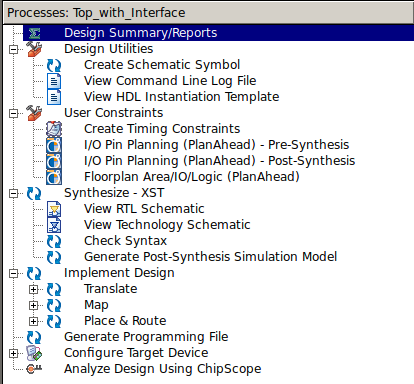
\includegraphics[width=0.7\linewidth]{img/verilog/ISE_HW_Generierungsfenster.png}
	\caption{Designflow im Hardware Generierungsfenster}
	\label{fig:gen_window}
\end{figure}

Zum Einen lässt sich unter \texttt{Synthesize {-} XST} > \texttt{View RTL Schematic} die Bereits aus vorherigen Beispielen RTL Schematic erzeugen. \\
\textbf{Hinweis:} Hierzu muss das Modul, welches untersucht werden soll, vorher als \texttt{TopModule} deklariert werden (Rechtsklick > \texttt{Set as Topmodule}).

\begin{figure}[H]
	\centering
	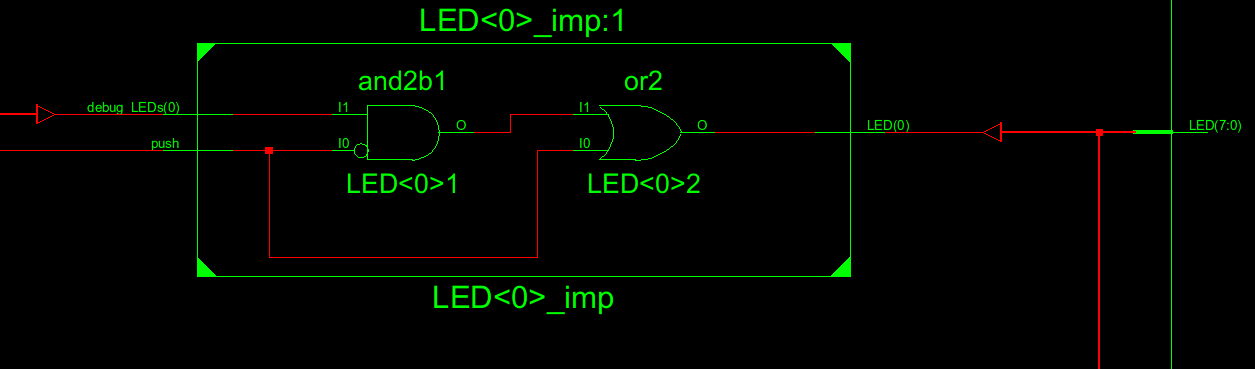
\includegraphics[width=\linewidth]{img/verilog/Schematic_RTL.png}
	\caption{Beispiel einer RTL Schematic}
	\label{fig:rtl_schematic}
\end{figure}

Des Weiteren findet man unter \texttt{Synthesize {-} XST} > \texttt{View Technology Schematic} die so genannte \texttt{Technology Schematic}.

\begin{figure}[H]
	\centering
	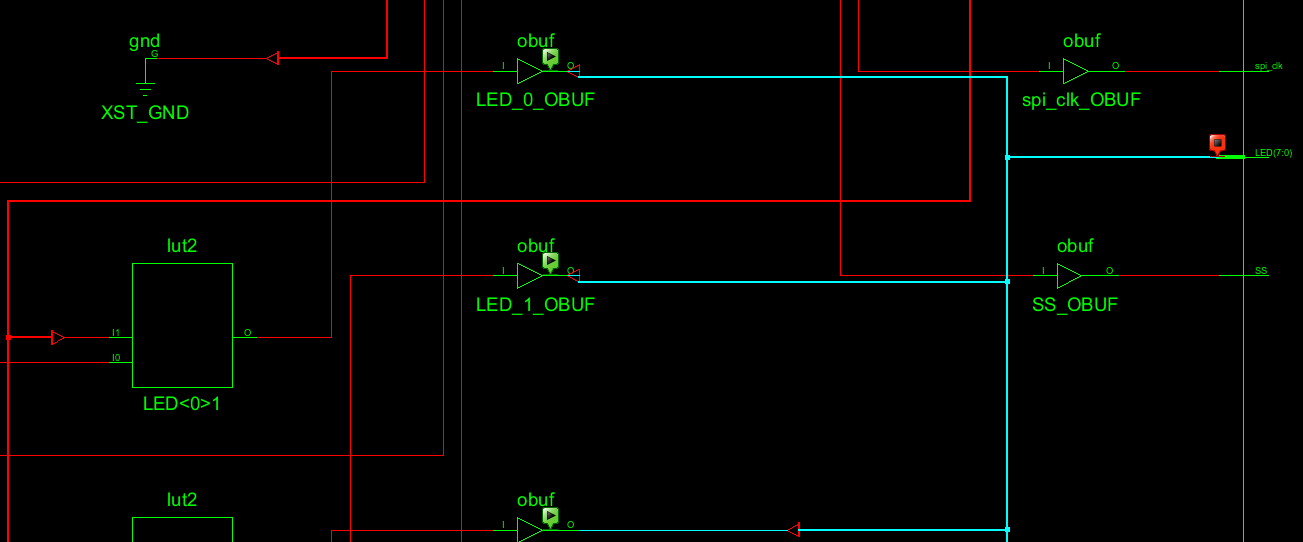
\includegraphics[width=\linewidth]{img/verilog/Schematic_Technology_Mapped.png}
	\caption{Beispiel einer Technology Schematic}
	\label{fig:tech_schematic}
\end{figure}

\subsubsection{Bitfile erstellen}
Funktioniert das Hardware-Design in der Testbench, geht es darum ein \texttt{Bitfile} zu erstellen und auf das FPGA zu laden. Dies verläuft ähnlich wie die Simulation, nur dass dieses Mal ein Doppelklick auf \texttt{Generate Programming File} in der \texttt{Implementation} Ansicht von Nöten ist. Hierbei ist zu beachten, dass das Topmodule ausgewählt sein muss und eine UCF Datei mit allen benötigten Constraints im Projekt vorhanden ist.


\subsubsection{Programmieren mit Bitfile}
Nach der erfolgreichen Synthese, Placing und Routing des Codes, erstellt ISE ein Bitfile in dem Projektverzeichnis. Dieses kann anschließend mit dem Kommandozeilen Tool \texttt{djtgcfg} auf das Board geladen werden. Auch wenn ISE dieses Feature selbst beinhaltet, verwenden wir hier dieses zusätzliche Programm, da es mehrere weitere Dinge ermöglicht von denen wir noch Gebrauch machen werden, wie zum Beispiel die Kommunikation mit dem Board im Betrieb.

\textbf{Schritt 1} (Finden des Boardnamens)\textbf{:}\\
Bevor das Board programmiert werden kann, muss überprüft werden, ob es angeschlossen ist und wie es benannt ist. Dafür wird auch das oben genannte Tool verwendet und die Liste der angeschlossenen Boards mit
\begin{center}
	\texttt{djtgcfg enum}
\end{center}
angezeigt. Das Wort hinter \texttt{Device:} ist der gesuchte Namen und wird im weiteren Verlauf als \texttt{<devicename>} referenziert. 

Falls es Probleme mit dem Erkennen gibt, kann ein erneutes Einstecken des USB-Kabels helfen.

\textbf{Schritt 2} (Erlangen weiterer Informationen)\textbf{:}\\
Wenn man den \texttt{<devicename>} des Boards kennt, lassen sich schnell weitere Informationen mittels
\begin{center}
	\texttt{djtgcfg init -d <devicename>}
\end{center}
erfragen. Falls hierbei die Meldung \texttt{ERROR: failed to initialize scan chain} in der Konsole erscheint, dann liegt es wahrscheinlich daran, dass das Board nicht eingeschaltet ist. Man darf sich außerdem nicht daran stören, dass eventuell mehrere Device IDs angezeigt werden.

\textbf{Schritt 3} (Programmieren)\textbf{:}\\
Während die ersten beiden Schritte nur je einmal ausgeführt werden müssen, muss dieser Schritt bei jeder Änderung des Bitfiles erneut ausgeführt werden. Der Befehl zum Übertragen des Bitfiles lautet:
\begin{center}
	\texttt{djtgcfg prog -d <devicename> -i 0 -f /absolute/path/to/file}
\end{center}
Hierbei ist zubeachten, dass der Pfad zum Bitfile absolut und nicht realtiv zum aktuellen Arbeitsverzeichnis sein sollte.

\subsection{\textsc{Versuch 3 und Aufgaben}}
Siehe Dokument zur Aufgabenstellung Kapitel 3.

\subsection*{Optionale Übung}
Eine weitere Aufgabe kann bei Interesse zur weiteren Vertiefung und Übung im Anhang \ref{sec:Taschenrechner} bearbeitet werden.